\chapter{Method}
\label{chap:method}

\section{Problem formulation}
\begin{comment}

Problem formulation, - state, action, what is our goal.
then with dynamics of quadrotor. 
After have PD controller under this.
Basic RL methods for this project
what use RL for in this project
Implementation
Experimental setup
\end{comment}

The task of this project is to evaluate the performance of DDPG and PPO as guidance systems in the context of quadrotor waypoint navigation.
Guidance in this case can be defined as “the process for guiding the path of an object towards a given point, which in general may be moving” \cite{shneydor1998Guidance} or ``a basic methodology concerned with the transient motion behavior associated with the achievement of motion control objectives'' \cite{Fossen2021}. As such, we can define the reinforcement learning objective as \textit{deciding the motion of a quadrotor through desired acceleration, such that it is able to reach a desired end position in 3-dimensional space.}

In a reinforcement learning context, the learning task thus becomes to discover an optimal policy that chooses an  action $A_t \in \mathcal{A}$ when in a state $S_t \in \mathcal{S}$, so that our state $S_t$ converges to some goal state as $t \rightarrow T$, where $T$ represents the end timestep of an episode. Our state and action is defined as:
\begin{equation}
    S_t = 
    \begin{bmatrix}
    \p_t^\top & \v_t^\top% x,y,z, u,v,w 
    \end{bmatrix} ^ \top, \qquad
    A_t = 
    \begin{bmatrix}
    \a_t
    \end{bmatrix}
    \label{4_1_stateActionsSpace}
\end{equation}
where $\p$, $\v \in \mathbb{R}^3$ denote the generalised position and velocity of the quadrotor with respect to the goal frame, $\{\text{goal}\}$, while and $\a$ denotes the acceleration of the quadrotor with respect to the body-fixed frame, $\{\text{b}\}$:
\begin{equation}
    \p_t^\text{goal} = \begin{bmatrix}
    x_t & y_t & z_t
    \end{bmatrix}^\top, \quad
    \v_t^\text{goal} = \begin{bmatrix}
    u_t & v_t & w_t
    \end{bmatrix}^\top, \quad
    \a_t^\text{b} = \begin{bmatrix}
    \Dot{u_t} & \Dot{v_t} & \Dot{w_t}
    \end{bmatrix}^\top
\end{equation}
Furthermore, the goal frame is stationary and represents an approximate inertial frame. The desired goal state is then chosen to be the origin of the goal frame, represented by the point $\p^\text{goal}_g = [0,0,0]^\top$.
From this, we see that the problem of waypoint navigation essentially becomes a task of setpoint regulation, where we wish to regulate our quadrotor position, $\p_t^\text{goal}$ to \textbf{0}.

As the reinforcement learning agents are responsible solely for the guidance of the quadrotor, we assume that there exists an underlying basic control system that is able to allocate the control inputs so as to produce the desired acceleration.
So, in the following section we will discuss how these accelerations are interpreted in the control system, before moving on to how we are able to implement the algorithms in practice and how exactly we will evaluate the DDPG and PPO algorithms.


\section{Dynamics of a Quadrotor}
\label{sec:4_dynamics}
In this section, we aim to cover the dynamics of the quadrotor through its rigid-body equations of motions, before moving on to the relationship between desired accelerations and generated forces in the feedback control system. Finally, we conclude with a description of the control allocation, showing how output torques from the control system is distributed to the individual rotors.

\subsection{Rigid-body Dynamics}
\label{sec:4_2_dynamics}
As the overall task of the reinforcement learning agent is to decide the motion of the quadrotor through acceleration, a natural first step is to understand how motion is achieved through the quadrotor rigid-body equations of motion.

To simplify notation, we define a right-hand inertial frame \{\textit{n}\} (e.g. the goal frame), and use \{\textit{b}\} to represent the the body-fixed frame as in the previous section. From \cite{MultirotorAerialVehicles} and using notation from \cite{Fossen2021}, we can then express the dynamics of the quadrotor as:
\begin{align}
    \Dot{\p}^n_{nb} &= \v^n_{nb} \\
    m \Dot{\v}^n_{nb} &= m\boldsymbol{g}^n + \boldsymbol{R} (\boldsymbol{\Theta}_{nb}) \, \boldsymbol{f}^b \label{4_1_transKinetics} \\ 
    \Dot{\boldsymbol{\Theta}}_{nb} &= \boldsymbol{\Theta}_{nb} \boldsymbol{\omega}^b_{nb_\times} \\
    \boldsymbol{I}^b_b\Dot{\boldsymbol{\omega}}^b &= - \boldsymbol{\omega}^b_{nb} \times \boldsymbol{I}^b_b\boldsymbol{\omega}^b_{nb} + \boldsymbol{\tau}^b  \label{4_1_rotKinetics}
\end{align}
\begin{table}[h]
    \centering
    \begin{tabular}{ll}
        $\boldsymbol{p^n_{nb}} \in \R^3$        & position of the quadrotor body-frame $\{b\}$ w.r.t. to $\{n\}$, expressed in $\{n\}$ \vspace{0.8mm} \\
        
        $\boldsymbol{v^n_{nb}} \in \R^3$        & velocity of the quadrotor body-frame $\{b\}$ w.r.t. $\{n\}$ expressed in $\{n\}$ \vspace{0.8mm} \\
        
        $m \in \R$                              & mass of the quadrotor \vspace{0.8mm} \\
        
        $\boldsymbol{g}^n \in \R^3$             &  gravitational acceleration $[0, 0, -g]^\top$, where \textit{g} = 9.81  ms$^{-2}$\vspace{0.8mm} \\
        
        $\boldsymbol{R} \in SO(3)$              & Euler angle rotation matrix from \{\textit{b}\} to \{\textit{n}\}, with argument $\boldsymbol{\Theta}_{nb}$ \vspace{0.8mm} \\
        
        $\boldsymbol{\Theta}_{nb} \in \R^3$     & orientation of the body-fixed frame \{\textit{b}\} w.r.t. \{\textit{n}\}, expressed with roll, \\ &pitch, yaw angles $[\phi, \theta,\psi]$ \vspace{0.8mm} \\
        
        $\boldsymbol{\omega}^b_{nb} \in \R^3$   & angular velocity of the quadrotor  body-frame $\{b\}$ w.r.t. $\{n\}$, expressed in $\{n\}$ \vspace{0.8mm} \\ 
        
        $\boldsymbol{\omega}^b_{nb_\times} \in \R^{3\times3}$ & skew-symmetric representation of $\boldsymbol{\omega}_{nb}$ \vspace{0.8mm} \\
        
        $\boldsymbol{I}^b_b \in \mathbb{R}^{3\times3}$ & inertia dyadic of the quadrotor body-fixed frame \{\textit{b}\}, expressed in \{\textit{b}\} \vspace{0.8mm} \\
        
        $\boldsymbol{f}^b \in \R^3$             & external forces applied to the quadrotor body frame $\{b\}$, expressed in \{\textit{b}\} \vspace{0.8mm} \\
        
        $\boldsymbol{\tau}^b \in \R^3$          & external moments applied to the quadrotor body frame $\{b\}$, expressed in \{\textit{b}\}
    \end{tabular}
    \caption{Notation used in the quadrotor rigid-body equations of motion.}
    \label{table:parameters}
\end{table}

Note that the subscripts $\{n\}$ and \{\textit{b}\} for $\Dot{\p}^n_{nb}$ and $\Dot{\v}^n_{nb}$ simply emphasise that the position and velocities are the movements of the body frame \{\textit{b}\} with respect to the inertia frame $\{n\}$, expressed in $\{n\}$, following from \cite{Fossen2021}. This is in contrast to Equation \eqref{4_1_stateActionsSpace}, where we denote $\Dot{\p}^n_t$ and $\Dot{\v}^n_t$ to show that these positions and velocities change with time.
The coordinate frames, along with the alignment of the body-fixed frame on the quadrotor can be seen in Figure \ref{fig:4_1_quadrotorBody}.
\begin{figure}[hbt]
    \centering
    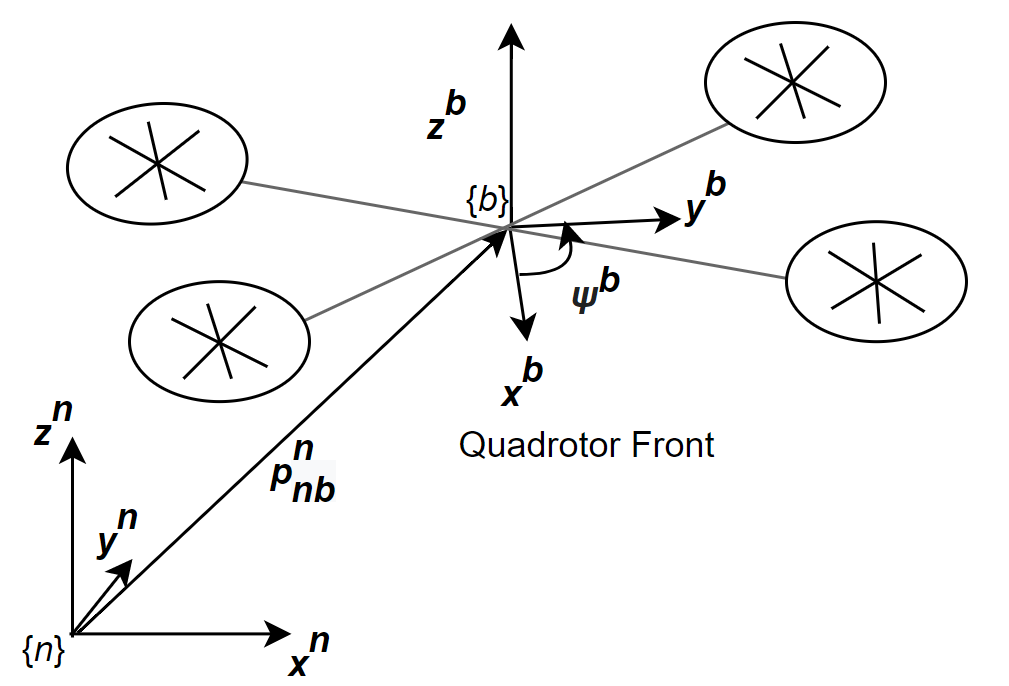
\includegraphics[width=0.7\textwidth]{figures/4_/4_2_quadrotorBody.png}
    \caption{An illustration of the relevant quadrotor coordinate frames. We have an inertial frame \{\textit{n}\} and a body frame \{\textit{b}\}.}
    \label{fig:4_1_quadrotorBody}
\end{figure}

Looking at equations of motion, we see a system with six degrees of freedom: three translational and three rotational. 
However, for a quadrotor, this means that we have an underactuated system. To illustrate this, the rotors have an arm that extends from the body-frame origin to the centers of each rotor. Since, these arms span the $\x^b\y^b$-plane and all of them produce a perpendicular thrust upwards along $\z^b$, we can mentally visualise that the quadrotor is able to produce torques to directly influence our roll $\phi$ and pitch $\theta$ angles, as well as a total force along $\z^b$. However, if our quadrotor body-frame \{$b$\} is aligned with the inertia frame \{$n$\}, all rotors produce a thrust parallel to $\z^n$ such that we cannot directly produce a vector thrust that spans the $\x^n\y^n$-plane, and hence our system is underactuated in these degrees of freedom. 

\begin{comment}
Formally, this is shown as \cite{Fossen2021}:
\begin{equation}
    \begin{bmatrix}
    \boldsymbol{f}^b \\
    \boldsymbol{\tau}^b
    \end{bmatrix}
    = \begin{bmatrix}
    \boldsymbol{f}^b \\
    \boldsymbol{r}^b_{tb} \times \boldsymbol{f}^b
    \end{bmatrix}
    = \begin{bmatrix}
    F_x \\
    F_y \\
    F_z \\
    l_y F_z - l_z F_y \\
    l_z F_z - l_x F_z \\
    l_x F_z - l_y F_x
    \end{bmatrix}
    \label{4_1_forceToThrust}
\end{equation}
where $\boldsymbol{r}^b_{tb} = [l_x, l_y, l_z]$ is the vector of lever arms from $\{b\}$ to the rotor centers, and $\boldsymbol{f}^b = [F_x, F_y, F_z]$ being the thrust vector decomposed in $\{b\}$ as before.
From this, we note that all degrees of freedom apart from 1 and 2 are non-zero, as $F_x$ and $F_y$ are zero. 
--In the hovering case, F_z is centered around the origin so all arms are 0. This means that only DOF 3 is non-zero so example could be confusing. 16/12
\end{comment}

So, to get be able to generate surge and sway velocities $u$ and $v$, the quadrotor has to exploit the system dynamics. Simply put, in order to accelerate along the $\x^n$ and $\y^n$ axes, the quadrotor can rotate its body-frame such that the overall thrust (along $\z^b$) points forward or sideways when decomposed $\{n\}$. This is shown in Equation \eqref{4_1_transKinetics}, where we see that accelerations $\Dot{\v}^n_{nb}$ in the inertial frame are proportional to the rotated force vector, $\boldsymbol{R} (\boldsymbol{\Theta}_{nb})\, \boldsymbol{f}^b$. For the sake of completeness, we can write this explicitly:
\begin{equation}
    \boldsymbol{R} (\boldsymbol{\Theta}_{nb}) = \begin{bmatrix}
    c\psi c\theta & -s\psi c\phi + c\psi s\theta s\phi & s\psi s\phi + c\psi s\theta c\phi \\
    s\psi c\theta & c\psi c\phi + s\psi s\theta s\phi & -c\psi s\phi + s\psi s\theta c\phi \\
    -s\theta &  c\theta s\phi & c\theta c\phi 
    \end{bmatrix}
\end{equation}
where, $c$ and $s$ refer to shorthand notations for sin and cos. Thus, if we denote $\boldsymbol{f}^b$ as $[0,0,F_z]^\top$, we can express accelerations $\dot u$ along $\x^n$ (roll $\phi$, yaw $\psi$ small), and $\dot v$ along $\y^n$ (pitch $\theta$, yaw $\psi$ small) as:
\begin{align}
    \dot u &= \frac{F_z}{m} \sin{\theta} \label{4_2_udot} \\
    \dot v &= - \frac{F_z}{m} \sin{\phi} \label{4_2_vdot}
\end{align}
From this, it is clear to see that to accelerate forward along $\x^b$, we have to command a positive rotation in pitch $\theta$, while to accelerate left along $\y^b$, we have to command a negative rotation in roll $\phi$. 

\subsection{Control Allocation}
With the overall relationship between forces and rotor thrust established, we can include a brief note on how the rotor thrusts relate to angular velocities.
As already hinted, the total thrust $T_\Sigma$ of a quadrotor can be represented as the sum of individual thrusts from each rotor:
\begin{equation}
    T_\Sigma = \sum^N_{i=1} |T_i| = c_T \sum^N_{i=1} \Bar{\omega}_i^2 \label{4_2_totalThrust}
\end{equation}
where,
\begin{equation}
    T_i = c_T \Bar{\omega}_i^2 = C_T \rho A_{r_i} r_i^2 \Bar{\omega}_i^2
\end{equation}
Here, $\Bar{\omega}_i$ is the angular velocity of rotor $i$ and $c_T$ is a product of some constant parameters: $C_T$ being the thrust coefficient, $\rho$ the density of air, $A_{r_i}$ the rotor disk area and $r_i$ the radius of rotor $i$. So, as mentioned before, by the geometry of the quadrotor we can express the force vector $\boldsymbol{f}^b$, as the overall thrust upwards along $\z^b$:
\begin{equation}
    \boldsymbol{f^b} = T_\Sigma \cdot \z^b + \Delta
\end{equation}
where $\Delta$ represents unmodelled aerodynamic forces when the rotor is not stationary \cite{MultirotorAerialVehicles}. 

Next, we can define the reaction torque acting on the quadrotor body, i.e. the rotational force experienced around $\z^b$, as:
\begin{equation}
    Q_i = c_Q \Bar{\omega}_i^2
\end{equation}
where $c_Q$ is a product of some constants similar to $c_T$ \cite{MultirotorAerialVehicles}. Quadrotors are designed such that every other rotor spins the opposite direction such that the sum of reaction torques are 0. The first rotor, $i=0$ (following from $\x^b$ going around $\z^b$) spins in an anti-clockwise positive rotation around $\z^b$, while the next spins clockwise and so on.

Lastly, as we are interested in commanding $\dot u$ and $\dot v$ accelerations through roll and pitch angles, we will have to consider the how torques around $\x^b$ and $\y^b$ are related to the rotor angular velocities $\Bar{\omega}_i$. This moment is given by the standard equation of a thrust $T_i$ multiplied by a lever arm $d_i$. Since the body-frame axes $\x^b,\y^b$ do not align with the airframe rotor-arm, we take the projection of these arms onto the  $\x^b,\y^b$ axes, where the angles between the axes and rotor-arms are $\pm$45$\degree$.

Knowing this, we can combine with \eqref{4_2_totalThrust}, and define $\boldsymbol{\tau} = \boldsymbol{B} \boldsymbol{\Bar{\omega}}$ such as:
\begin{equation}
    \begin{bmatrix}
        T_\Sigma \\ \boldsymbol{\tau}^b
    \end{bmatrix}
    = \begin{bmatrix}
        T_\Sigma \\ \tau_1 \\ \tau_2 \\ \tau_3
    \end{bmatrix}
    = \underbrace{
        \begin{bmatrix} 
            c_T & c_T & c_T & c_T \\ 
            d\frac{\sqrt{2}}{2} & d\frac{\sqrt{2}}{2} & -d\frac{\sqrt{2}}{2} & -d\frac{\sqrt{2}}{2} \\ 
            -d\frac{\sqrt{2}}{2} & d\frac{\sqrt{2}}{2} & d\frac{\sqrt{2}}{2} & -d\frac{\sqrt{2}}{2} \\ 
            -c_Q & c_Q & -c_Q & c_Q 
        \end{bmatrix}
    }_{\boldsymbol{B}}
    \begin{bmatrix}
    \Bar{\omega}_1^2 \\
    \Bar{\omega}_2^2 \\
    \Bar{\omega}_3^2 \\
    \Bar{\omega}_4^2 \\
    \end{bmatrix}
    \label{4_2_controlAllocation}
\end{equation}
From this, we can find the angular velocities $\boldsymbol{\Bar{\omega}}$, for a desired set of torques and thrust $\boldsymbol{\tau}$, by taking the inverse of the control allocation matrix $\boldsymbol{B}$ and solving the inverse equation $\boldsymbol{\Bar{\omega}} = \boldsymbol{B}^{-1} \boldsymbol{\tau}$.  


\section{Role of Reinforcement Learning}

Now the quadrotor dynamics is understood, we can look into how reinforcement learning will be used specifically. As mentioned, our action space in \eqref{4_1_stateActionsSpace} is the acceleration vector $\a^b_t$ expressed in the body frame, $\{b\}$. Essentially, this is indirectly achieved by commanding a roll $\phi$ and pitch $\theta$ angle, as shown in \eqref{4_2_udot}, \eqref{4_2_vdot}. The relationship made between the desired acceleration and the roll and pitch angles is done in the basic control layer -- the PD controller -- which then uses the rotational kinetics in \eqref{4_1_rotKinetics} and the control allocation in \eqref{4_2_controlAllocation}, to produce the correct rotor angular velocities.

Conventionally, this means that our reinforcement learning agent represents an optimal control layer, or optimal controller, that serves as a guidance system that determines the optimal next-states in the waypoint navigation task. This makes sense as the reinforcement learning problem can be expressed as an optimisation problem, when considering large state-action spaces as mentioned in Section \ref{sec:2_6_modelFreeContinuous}. 
\begin{figure}[ht]
    \centering
    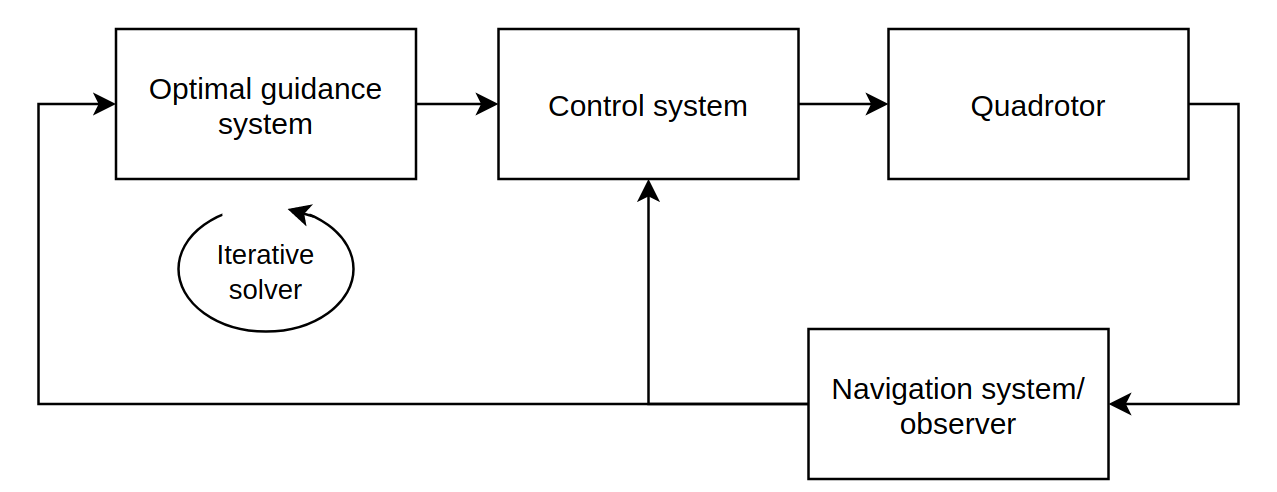
\includegraphics[width=0.8\textwidth]{figures/4_/4_1_Guidance.png}
    \caption{Traditional optimal trajectory generation using an iterative solver to an optimisation problem. Recreated from \cite{Fossen2021}.}
    \label{fig:4_3_Guidance}
\end{figure}
\begin{figure}[ht]
    \centering
    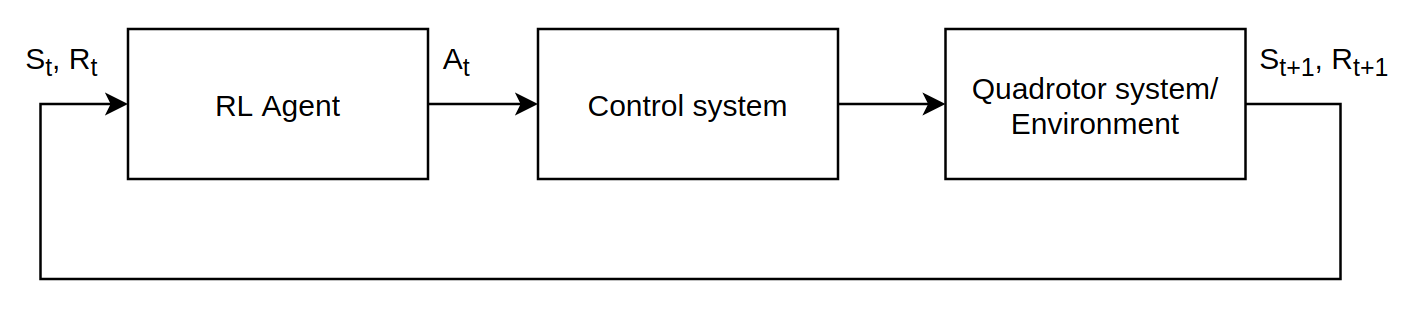
\includegraphics[width=0.9\textwidth]{figures/4_/4_1_RLGuidance.png}
    \caption{Using the reinforcement learning agents, DDPG and PPO, as optimal guidance systems that send accelerations (roll, pitch and height references) to the control system.}
    \label{fig:4_3_RLGuidance}
\end{figure}

Figure \ref{fig:4_3_Guidance} shows the classic setup of a guidance, navigation and control system, where the optimal trajectory is can be generated through a minimisation of a specific cost function, such as in quadratic programming (QP). Moving on, we see that the role of our DDPG and PPO algorithms will be to undertake the guidance system, such that our overall system transforms to Figure \ref{fig:4_3_RLGuidance}.

It is also not uncommon to use reinforcement learning agents to replace both guidance and control systems, such that the agents have to learn the mapping from their states $S_t$ to individual rotor thrusts $T_i$. This is for example done in \cite{ControlofQuadrotorRL} and \cite{song2021droneRacing}, where they have achieved excellent results. Otherwise, in \cite{PPOQuadrotor}, a step further was taken as states were mapped directly to rotor angular velocities. Nonetheless, we do not follow these approaches, but choose rather to utilise the underlying PD-controller. This makes our state and action spaces most alike \cite{RodriguezRamos2019ADR}, though ours is extended to three dimensional space.

The benefit of having a ``high'' abstraction output is that the learning task becomes more simplified as there are less physical relationships that needs to be learned. Instead, a PD controller can be used to leverage the underlying dynamics as we have good models for these. The downside however, is that through commanded accelerations we assume that the roll and pitch angles represent their desired values: $\phi = \phi_d$ and $\theta = \theta_d$. This entails that there must be a significant bandwidth separation between the reinforcement learning agent ``action frequency'' and the closed-loop control system bandwidth, so that this expectation is realistic. However, this is a possible limitation in the performance of the reinforcement learning agent as it cannot react as quickly to disturbances.

\section{Implementation}
In this section, we will look into how we can compare the DDPG and PPO algorithms from a practical perspective. To do this, we will look into how guidance and control of a quadrotor can be done through simulation, using a physics-based simulator called Gazebo \cite{Gazebo}.
Specifically, we will look into the different modules that are a part of the Gazebo framework, starting first with our quadrotor, then how this can be simulated, and finally how the algorithms are integrated into this system. Lastly, we will see how these modules are integrated into one complete system using the Robot Operating System (ROS).

The quadrotor used during this project is a model of the resilient micro-flyer (RMF), which is a collision-tolerant quadrotor well suited for navigation in a confined environment. The quadrotor can be visualised in Figure \ref{fig:4_1_rmf} below.
\begin{figure}[hbt]
    \centering
    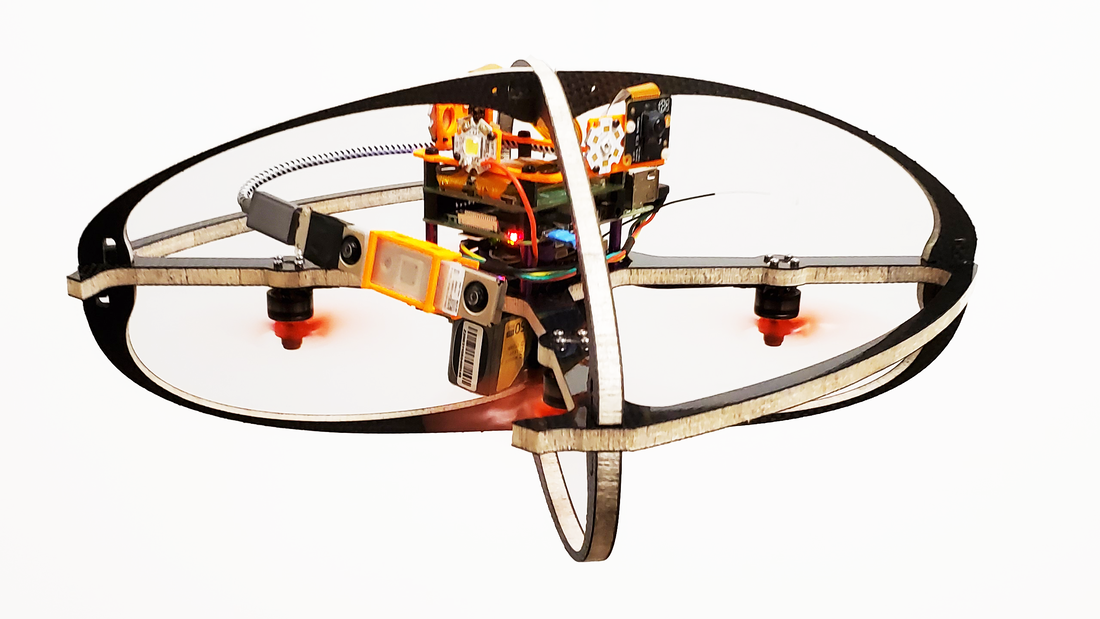
\includegraphics[width=0.5\textwidth]{figures/4_/rf-side-view-free-flight_orig.png}
    \caption{An image of an actual RMF, taken from \href{https://www.autonomousrobotslab.com/}{Autonomous Robots Lab}}
    \label{fig:4_1_rmf}
\end{figure}


\subsection{Gazebo}

The Gazebo \cite{Gazebo} physics-based simulation framework serves as a more realistic alternative compared to other simpler reinforcement learning environments, such as OpenAI Gym or Atari-based games. It allows its users to create models of their own robotic system, with custom sensors and actuators added, where it is then able to determine the dynamical response for this system given some external or control forces. This makes it an ideal choice for researchers looking to develop and test their algorithms, without requiring or risking a real robotic system.

To be able to simulate the RMF quadrotor seen in Figure \ref{fig:4_1_rmf}, we use a combination of a micro aerial vehicle (MAV) simulator, namely the \textit{RotorS} extension \cite{RotorS_Furrer2016}, together with some RMF Unified Robotic Description Format (URDF) files, to yield an RMF simulator.
The RotorS extension is a quadrotor simulator that the contains a variety of elements, such as an IMU, generic odometry sensor, visual-inertial sensor, autopilot, along with some quadrotor models \cite{RotorS_Furrer2016}.
The URDF files contains information about the RMF specific sensors, shape, weight, etc., describing all elements of the RMF.
Thus, by creating a workspace that includes these extensions, we then achieve a RMF simulator that is able to run fast and accurate simulations of the RMF quadrotor, risk-free.

But before we are able to command the quadrotor through RotorS, we need a way to do reinforcement learning with this system. If we recall from section \ref{chap:background_RL}, we essentially need an MDP environment for which the agent can perform actions in. As such, we used a wrapper for RotorS that served as both an environment and a method to communicate with the simulator. 
This wrapper allowed us to emulate a typical OpenAI gym environment, which then made it possible to use OpenAI's baseline implementations of DDPG and PPO \cite{baselines}.

So finally, we have a system where the agent, the DDPG or PPO algorithms, is able to interact with the RMF quadrotor environment through a RotorS wrapper, which further communicates the agent's decisions via messages to the simulator.
\begin{figure}[htb]
    \centering
    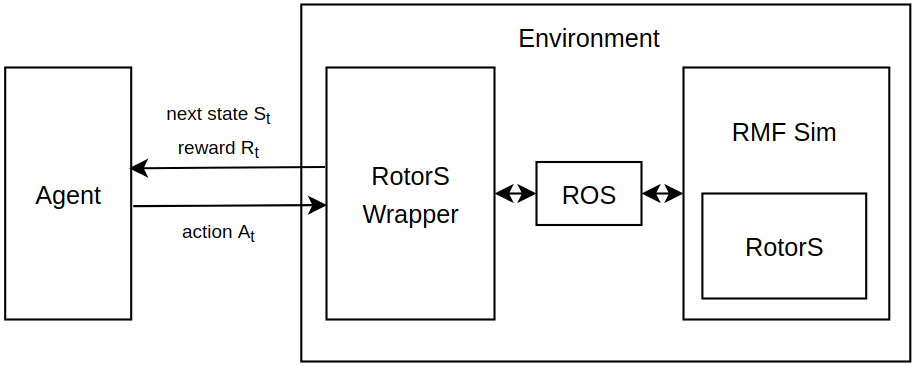
\includegraphics[width=0.85\textwidth]{figures/4_/4_1_simFramew.png}
    \caption{A diagram showing the overall simulation framework of our system, where different modules communicate via ROS.}
    \label{fig:4_1_simFramework}
\end{figure}


\subsection{ROS}
With the different components of the framework listed, what remains is the method of communication between these. The Robot Operating System (ROS) serves this purpose, being a middleware for robotics software \cite{ROS}. It is essentially a form of standardised communication, where different \textit{nodes} can communicate with each other, sending \textit{messages} via \textit{topics}. In this case, a node is simply an executable file that listens to or sends messages, by \textit{subscribing} and \textit{publishing} to a topic, respectively. A node can also offer a service, which will simply execute some function. 

ROS standardises the way that message passing occurs by using strictly typed data structures as messages which allows the type and content of a message to be easily identified. Similarly, topics are like message channels which allow us to quickly identify which nodes communicate with each other. These topics also allow new nodes to obtain messages it finds interesting by subscribing to those topics, without having to make any changes on the publisher side.

So, for this project, ROS is used as a way to integrate RotorS with the RMF module, but also as a method for the agent to communicate with the RMF Simulator, as seen in Figure \ref{fig:4_1_simFramework}.
In our case, the agent is directly able to communicate with the RotorS wrapper as they both exist in the same ROS package. 
The RotorS wrapper then serves as an environment interface, which receives odometry messages from, and sends thrust messages to, the RMF simulator.



\section{Experimental Setup}
\label{sec:4_5_experimentalSetup}

In this section, we go through the different design choices of the experiment, beginning with the reward function, before moving on the how the network is structured and how training is set up. Then, in Section \ref{sec:4_Experiment}, we will move on to the actual experiment of changing the \textit{hyperparameters} of the network and evaluating the effect this has on the performance of the DDPG and PPO algorithms.

\subsection{Reward Function}
\label{subsec:4_5_rewardFunction}

The reward function is one of the most important design tools within reinforcement learning. Through the choice of reward structure, one can indirectly manipulate the learned agent behaviour to match the behaviour we hope to observe during testing. Though conversely, having such a delicate tool may be a burden in disguise. The complex behaviour that an agent learns is based directly on the idea of maximising the total reward, by means of exploiting the environment, but also the reward function. Hence, any unmet expectations in the agent performance can often be the consequence of a poorly designed reward function.

For the purpose of waypoint navigation, we can construct a reward function that minimises the distance between the goal and the quadrotor, while  also maintaining a reasonable speed. We can add an additional goal reward to this function, which signals that the agent has been successful in reaching its goal.
The reward structure chosen is a quadratic reward function, inspired by the QP-problem formulation in optimal control. The reward function then resembles a cost function, penalising position, velocity and acceleration, with a goal reward $G$:
\begin{equation}
    R \, (S_t, A_t) = - S_t^\top \boldsymbol{Q} S_t -  A_t^\top \boldsymbol{R}  A_t  + G(S_t)
    \label{4_rewardFunction}
\end{equation}
Our states $S_t$ and actions $A_t$ are defined as in \eqref{4_1_stateActionsSpace} and the $\boldsymbol{Q}$ and $\boldsymbol{R}$ matrices represent the weighting for each element of the state and action. Explicitly, the reward can be written as:
\begin{equation}
R \, (\p_t, \v_t, \a_t) = - 
    \begin{bmatrix}
    x_t, y_t, z_t, 
    u_t, v_t, w_t
    \end{bmatrix}^\top
    \boldsymbol{Q}
    \begin{bmatrix}
    x_t\\
    y_t\\
    z_t\\
    u_t\\
    v_t\\
    w_t
    \end{bmatrix}
    -
    \begin{bmatrix}
    \Dot{u_t}, \Dot{v_t}, \Dot{w_t}
    \end{bmatrix}^\top
    \boldsymbol{R}
    \begin{bmatrix}
    \Dot{u_t}\\
    \Dot{v_t}\\
    \Dot{w_t}
    \end{bmatrix}
    + G(S_t)
\end{equation}
where,
\begin{equation}
    \boldsymbol{Q} = \frac{1}{250}
    \begin{bmatrix}
    0.6 & 0 & 0 & 0 & 0 & 0 \\
    0 & 0.6 & 0 & 0 & 0 & 0 \\
    0 & 0 & 1.0 & 0 & 0 & 0 \\
    0 & 0 & 0 & 0.03 & 0 & 0 \\
    0 & 0 & 0 & 0 & 0.03 & 0 \\
    0 & 0 & 0 & 0 & 0 & 0.05 
    \end{bmatrix}, \quad
    \boldsymbol{R} = \frac{1}{250}
    \begin{bmatrix}
    0.001 & 0 & 0 \\
    0 & 0.001 & 0 \\
    0 & 0 & 0.001
    \end{bmatrix}
    \label{4_QR_rewardWeights}
\end{equation}
and,
\begin{equation}
    G\,(S_t) =
    \begin{cases} 
      1 & \text{if} \,\, || \p_t || < 0.25 \,\, \text{and}\,\, || \v_t || < 0.3 \\
      0 & \text{otherwise}
    \end{cases}
    \label{4_goal_condition}
\end{equation}
Based on this reward function, the agent should be primarily motivated to reduce its position relative to the goal, but also with low speeds and without the use of excessive acceleration.
The goal reward serves the purpose to speed up the learning process, where it offers additional positive feedback so that the agent will know to repeat its actions. Further, we specify that the goal, $G(S_t)$, is reached if the quadrotor is able to stay within a goal radius of 0.25m with a total velocity of less than 0.3ms$^{-1}$. 

The weighting matrices $\boldsymbol{Q}$ and $\boldsymbol{R}$ describes the ``cost'' of each element, such that larger values correlate to more prioritised states and more expensive actions.
We can also note that the $z$ term is weighted more than the $x$ and $y$ terms in $\boldsymbol{Q}$. This choice is physically motivated by the fact that a quadrotor is more easily (directly) able to control its height rather than its lateral position, as shown in Section \ref{sec:4_2_dynamics}. Also, when considering that lateral accelerations require a change in the roll and pitch angles, this can result in unwanted changes to the quadrotor height. So, by having a more prioritised $z$ term, we wish that commanding the $\dot u$, $\dot v$ accelerations does not affect the height, $z$.

Another important consideration for the weighting matrices is that they should reflect the dynamics of the system. From \cite{song2021droneRacing}, we see that the inertial matrix for a quadrotor can be represented with a diagonal matrix $\boldsymbol{J} = [0.003, 0.003, 0.005]$ kg m$^2$, which is also provides a good justification for our chosen reward function.


\subsection{Network Architecture}
\label{sec:4_5_networkArchitecture}

In this section, we will look into the NN structure used for DDPG and PPO, and how these models are optimised. Recall from Chapter \ref{chap:3_Optimisation} that we can use NNs as function approximators that parametrise the policy $\pi$ and action-value function $Q$ (or value function $V$) in actor-critic algorithms.

\subsubsection{Network Types}
The most commonly used NN model is a fully-connected neural network (NN), which is also (ambiguously) referred to as a \textit{multi-layer perceptron} (MLP) in the reinforcement learning community. These models are the most conventional type of network, where each neuron in one layer is connected to every other neuron in the next layer.
There are also other model types that have been utilised, such as convolutional NNs (CNNs) in \cite{DQN}, or recurrent NNs (RNNs) like in \cite{Chen2016DRQN} that builds on \cite{DQN}. Generally, if we are dealing with structured data a CNN is most appropriate, while for data with a temporal relationship an RNN is beneficial. This being said, if our states hold the Markov property -- in contrast to partially observed MDPs (POMDPs) -- standard NNs are more than suitable as all the information in the previous states can be deduced from the current state.

\subsubsection{Network Choice}
So, in this project, we will be utilising fully-connected NNs to parametrise the policy and value functions. For DDPG, both networks have two hidden layers, where the width is a design parameter for this project, as described in Section \ref{sec:4_Experiment}. The Actor-Critic structure for DDPG is shown in Figure \ref{fig:4_3_networkArchitecture}. Note that for the DDPG algorithms, we have also target networks for both the actor and critic network with identical size, such that we have a total of four networks.
\begin{figure}[htb]
    \centering
        \begin{subfigure}[b]{.49\textwidth}
        \centering
        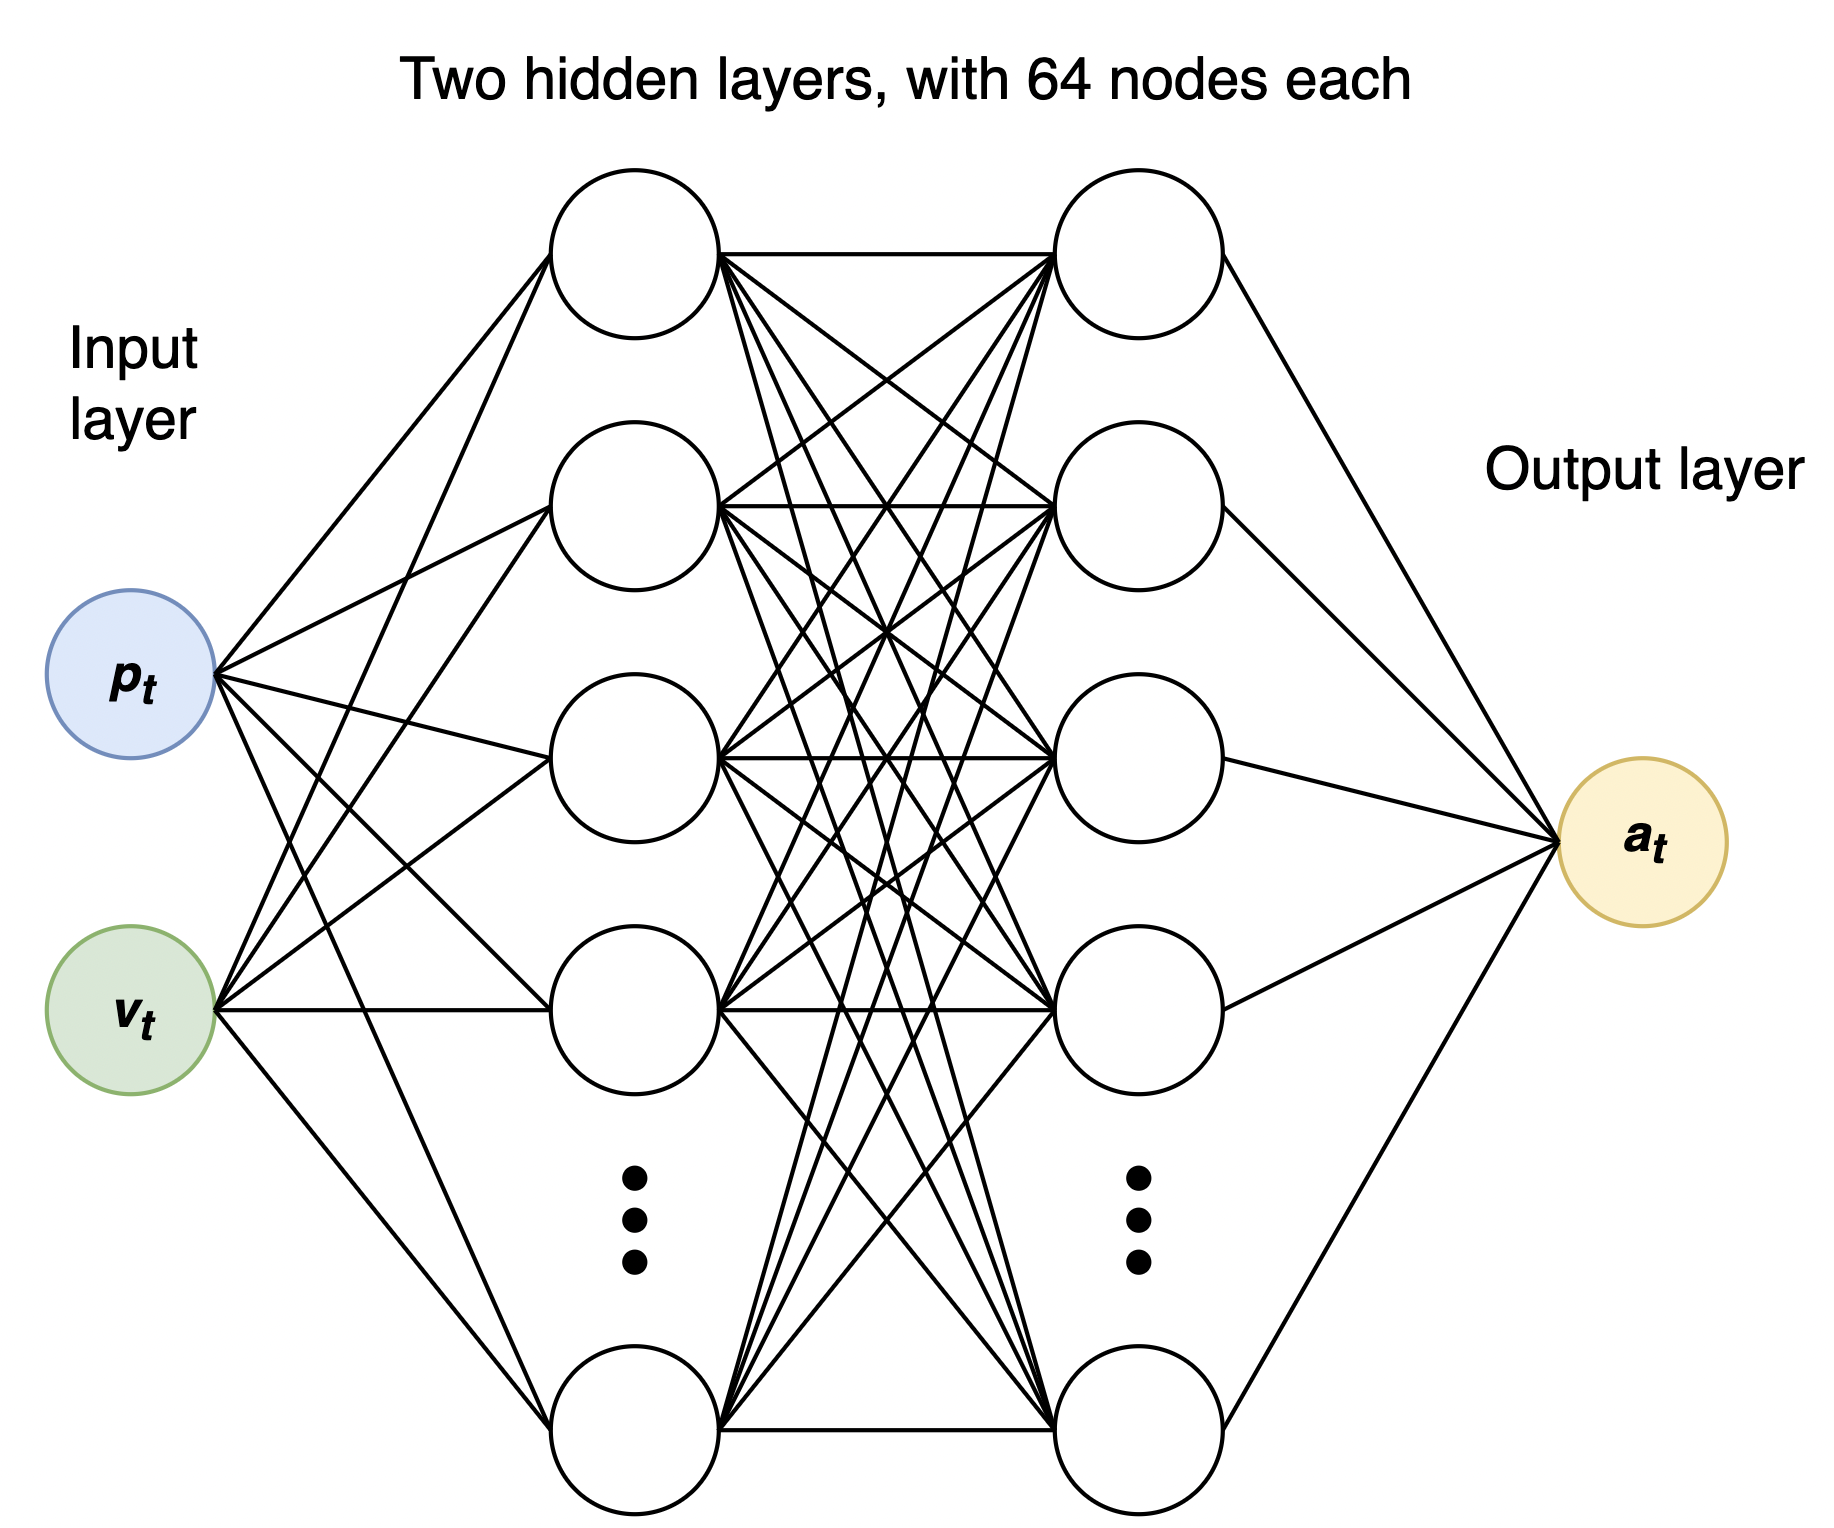
\includegraphics[width=.95\textwidth]{figures/4_/4_5_actor.drawio-labelled.png}
        \caption{Actor model with weights $\btmu$. The actor takes an input state $s \in \mathbb{R}^6$ comprising of a \textcolor[HTML]{004CD9}{position} $\p_t$ \textcolor[HTML]{009900}{velocity} $\v_t$ vector, to output an \textcolor[HTML]{D6C415}{acceleration} $\a_t  \in \mathbb{R}^3$ as action $a = \pi(s | \btmu)$.}
        \label{fig:4_3_actor}
    \end{subfigure}
    \hfill
    \begin{subfigure}[b]{0.49\textwidth}
        \centering
        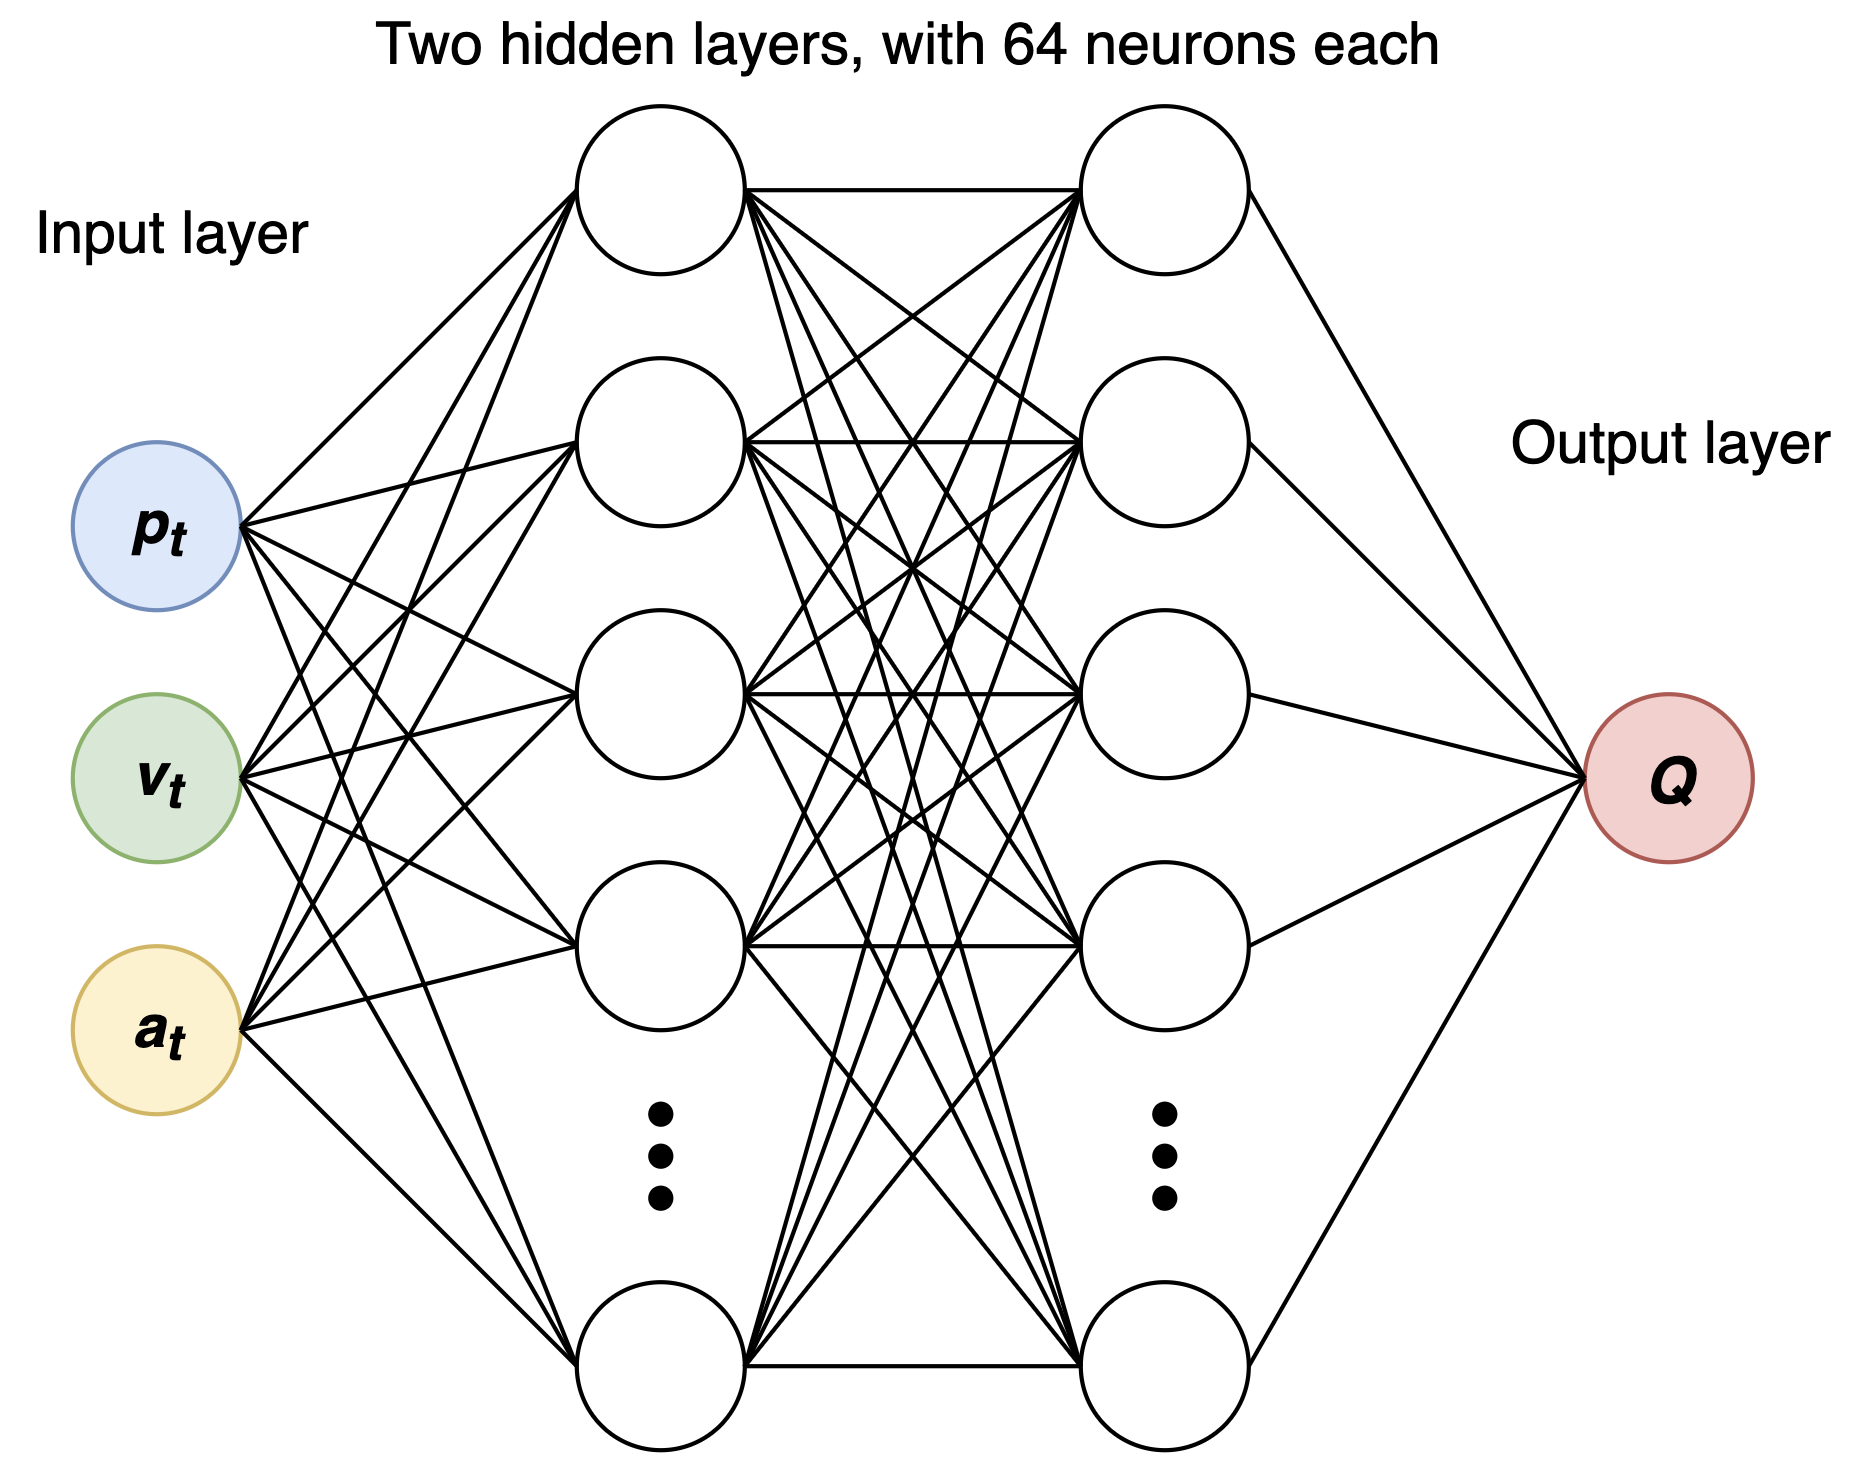
\includegraphics[width=.95\textwidth]{figures/4_/4_5_critic.drawio.png}
        \caption{Critic model with weights $\btQ$. The critic takes the concatenated state-action pair $[\p_t, \v_t, \a_t] \in \mathbb{R}^9$ as input, and yields the \textcolor[HTML]{CC262A}{estimated return} $Q(s,a | \btQ) \in \mathbb{R}$ for that pair, under some policy $\pi$.}
        \label{fig:4_3_critic}
    \end{subfigure}
    \hfill
    \caption{An overview of the actor and critic network architecture for DDPG.}
    \label{fig:4_3_networkArchitecture}
\end{figure}
\begin{figure}[hbt]
    \centering
        \begin{subfigure}[b]{.55\textwidth}
        \centering
        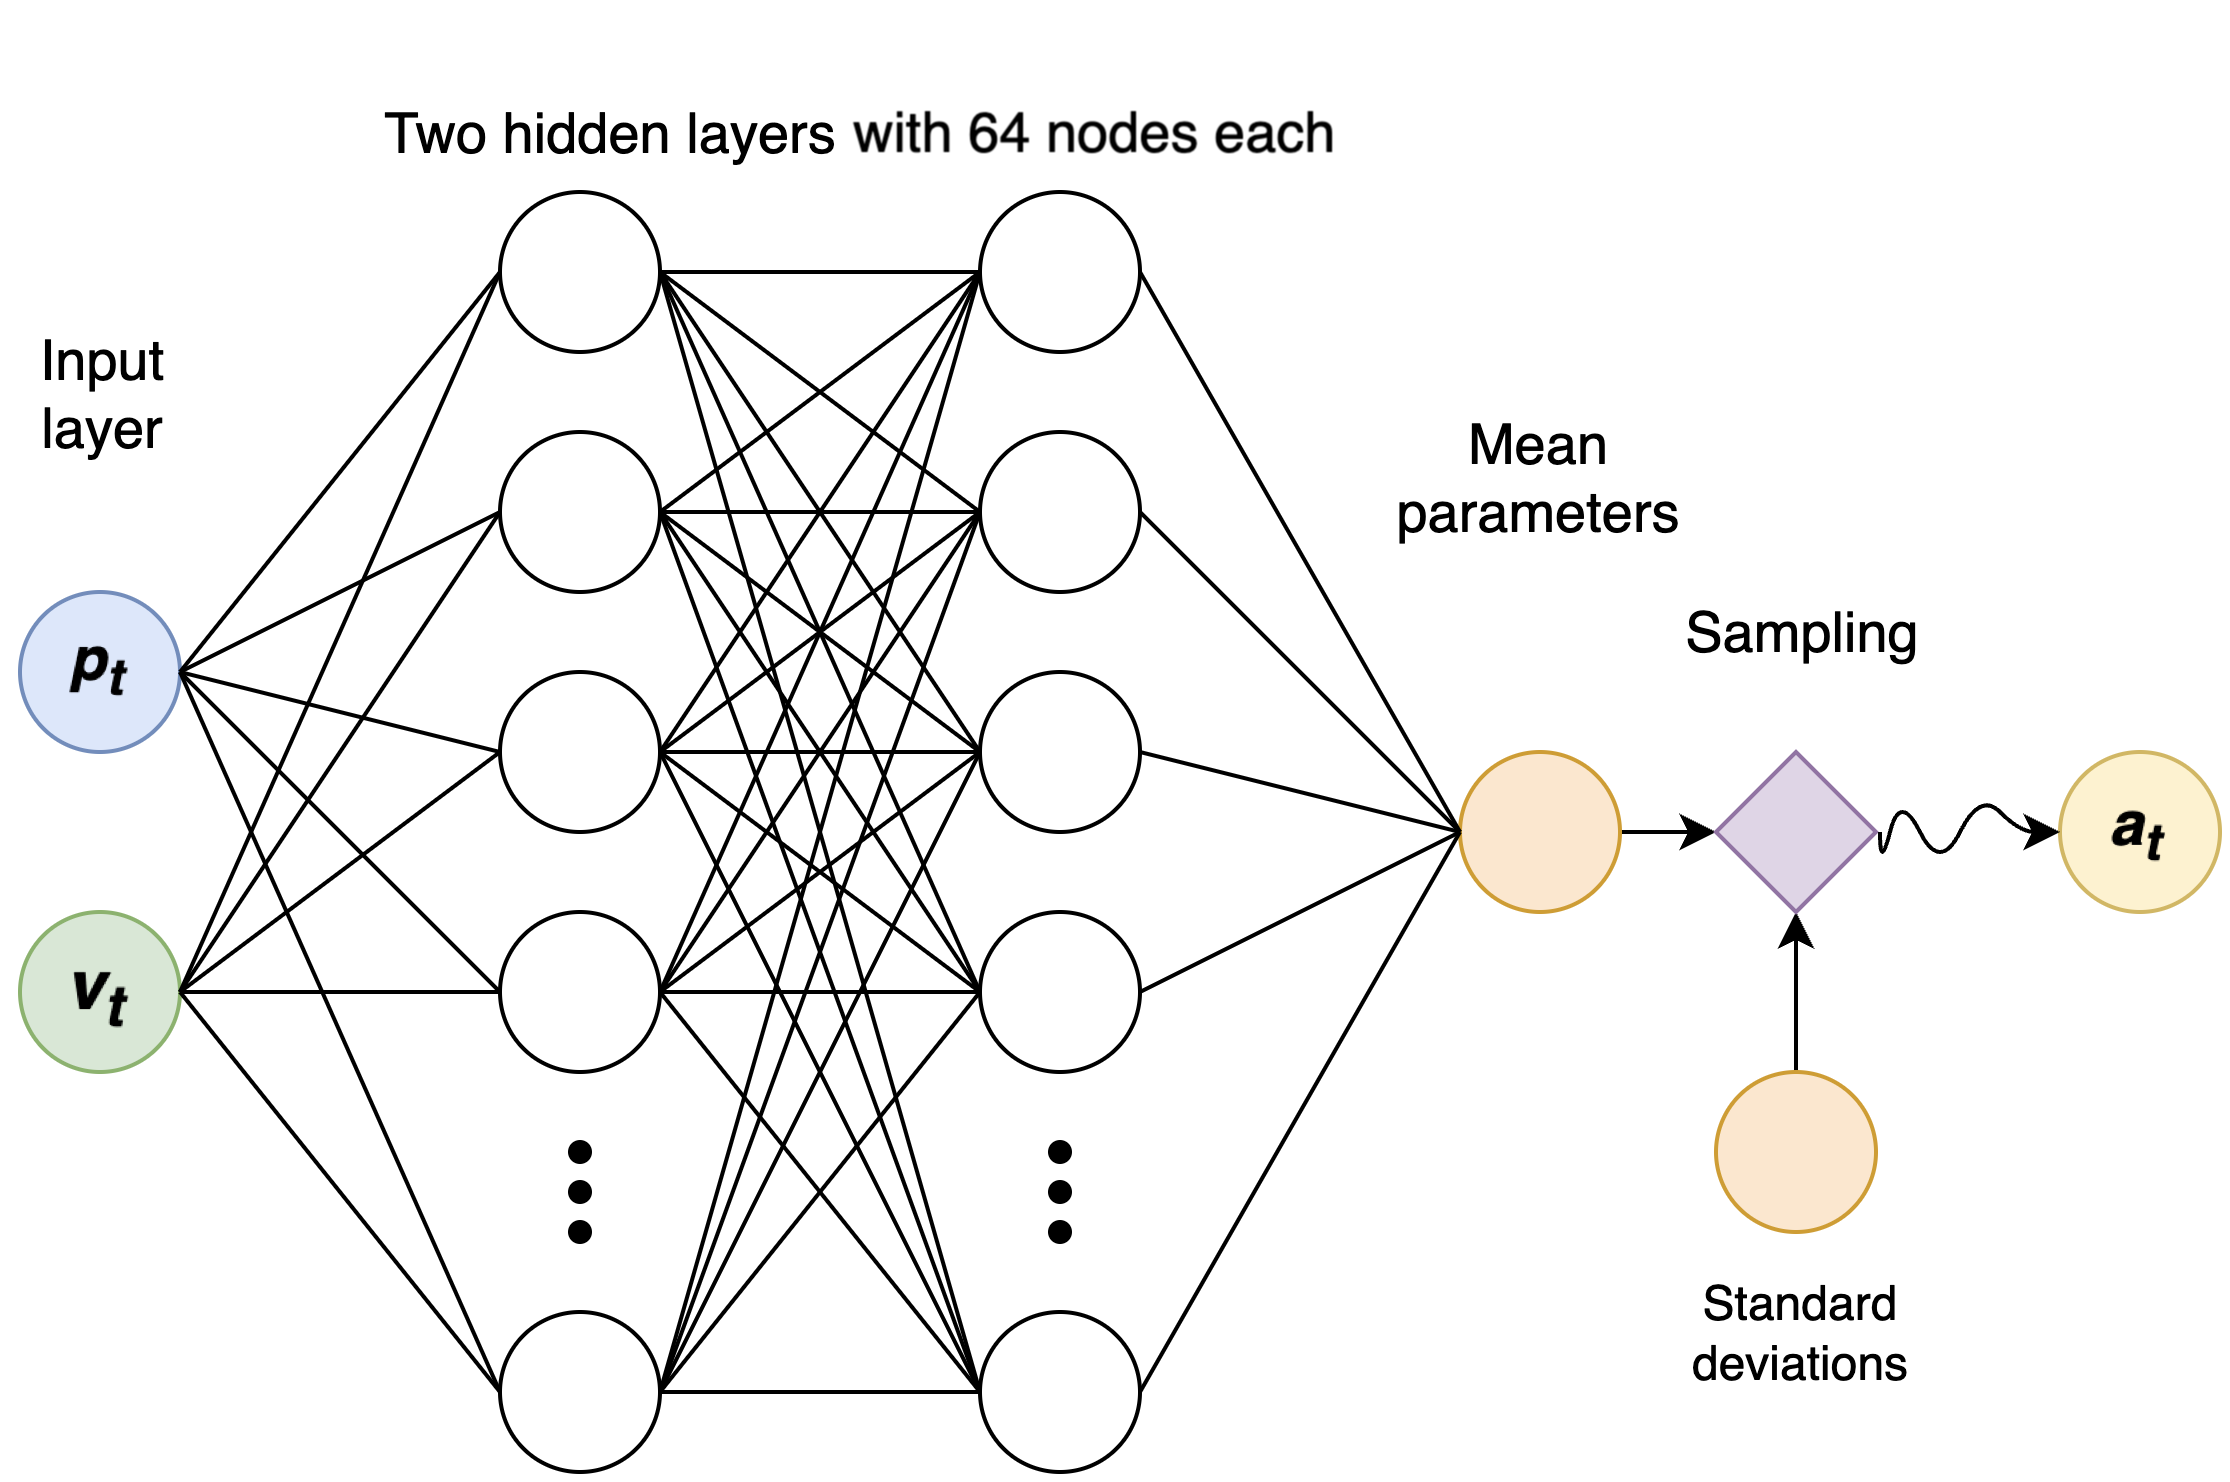
\includegraphics[width=.95\textwidth]{figures/4_/4_5_actor_ppo.drawio.png}
        \caption{Actor model with weights $\bt$, parametrising a stochastic policy $\pibt$. The actor takes an input state $s \in \mathbb{R}^6$ comprising of a \textcolor[HTML]{004CD9}{position} $\p_t$ \textcolor[HTML]{009900}{velocity} $\v_t$ vector, to output Gaussian distribution \textcolor[HTML]{DA8A67}{parameters} $\in \mathbb{R}^{3\times2}$, from which the \textcolor[HTML]{D6C415}{action} $\a_t \in \R^3$ is sampled.}
        \label{fig:4_5_PPOactor}
    \end{subfigure}
    \hfill
    \begin{subfigure}[b]{0.44\textwidth}
        \centering
        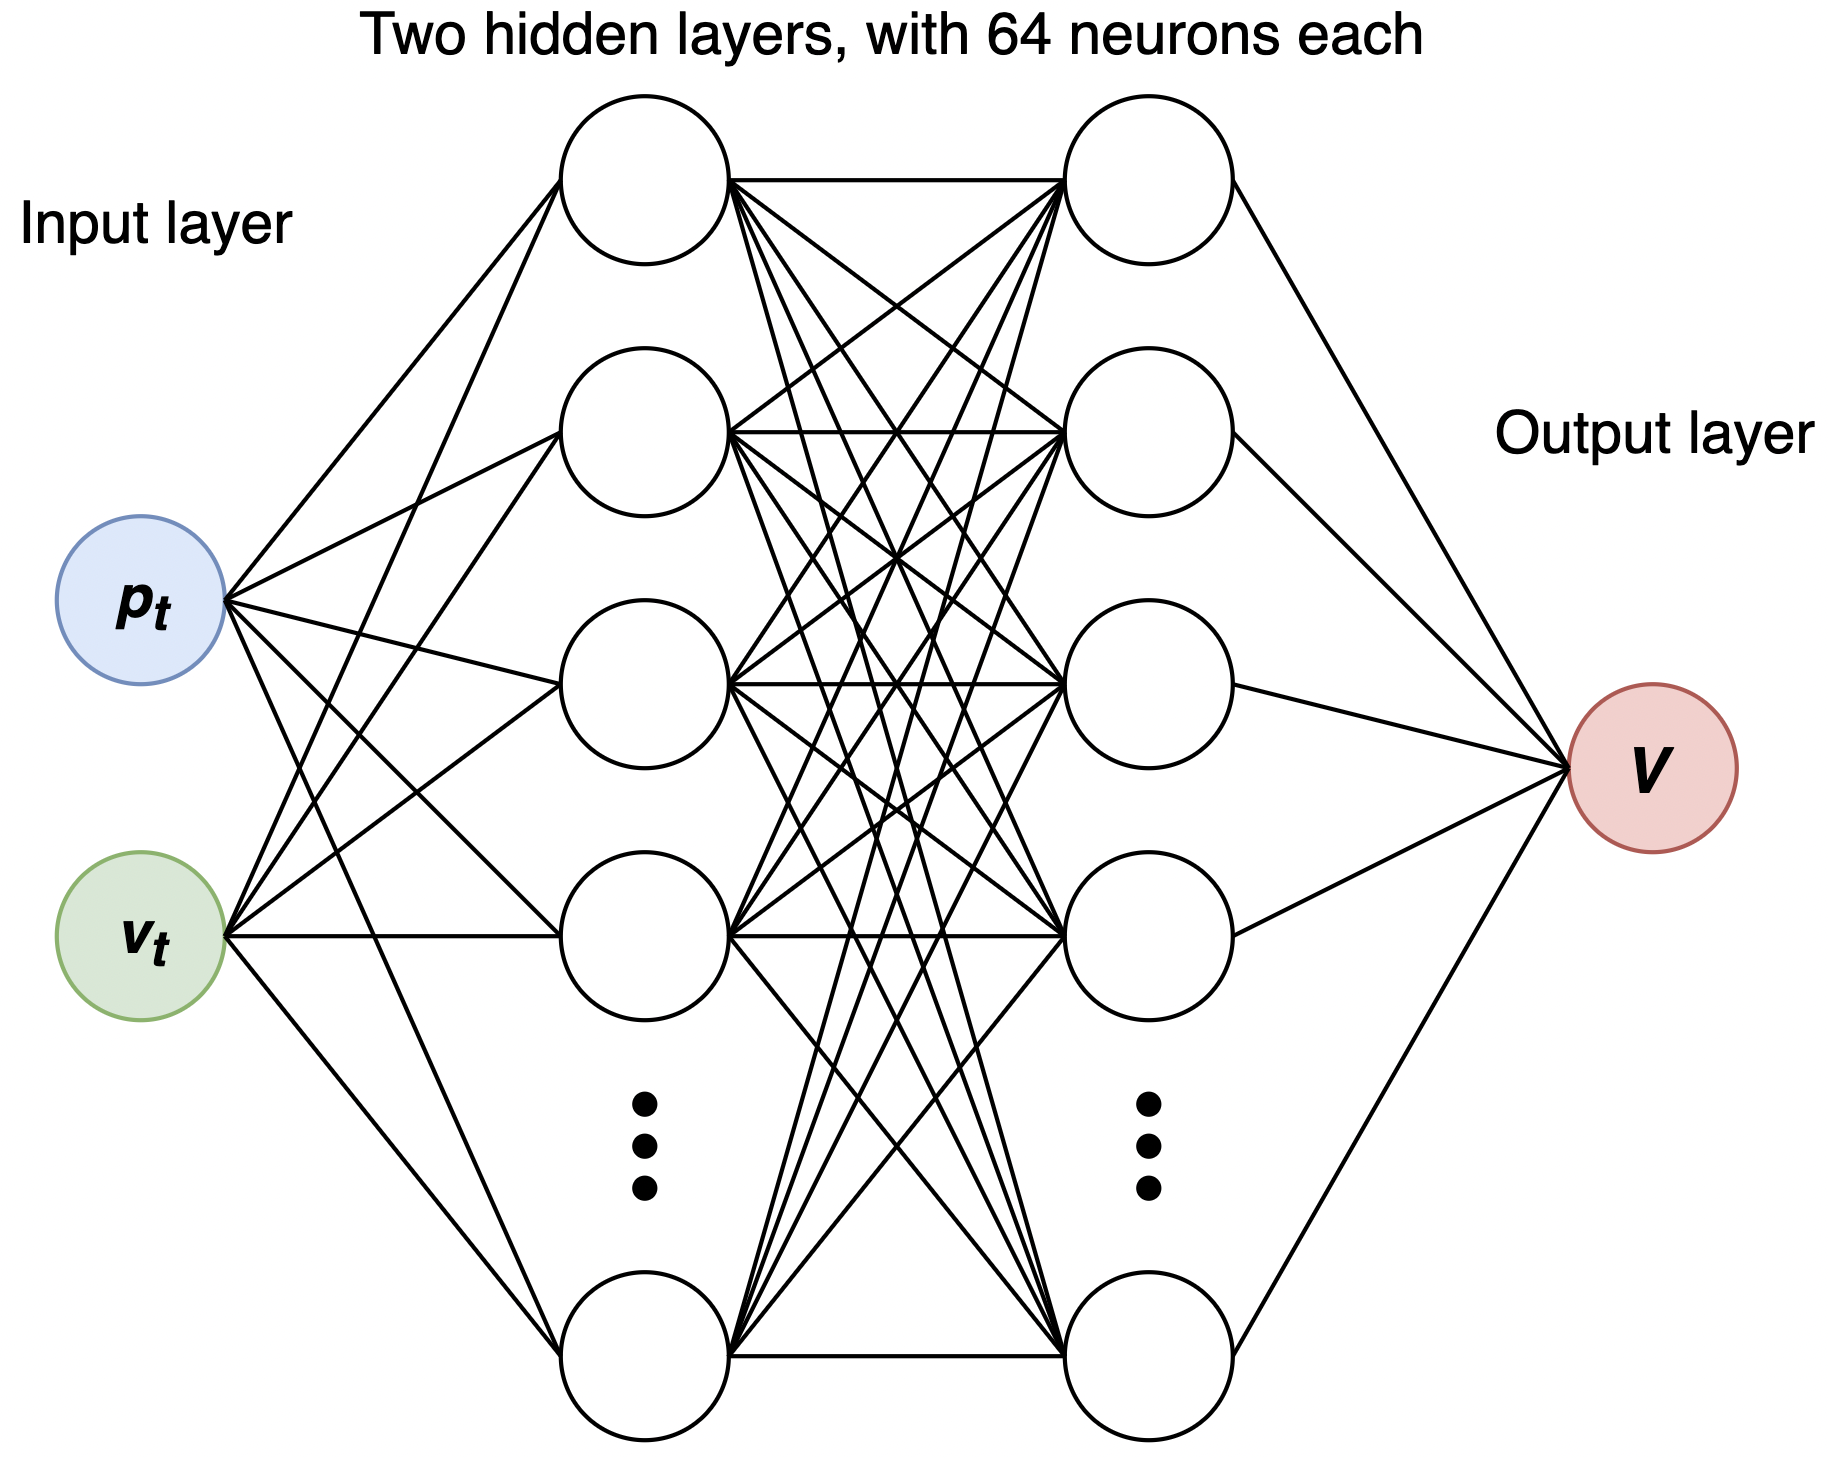
\includegraphics[width=.95\textwidth]{figures/4_/4_5_critic_ppo.drawio.png}
        \caption{Critic model also with weights $\bt$. The critic takes the state $[\p_t, \v_t] \in \mathbb{R}^6$ as input, to yield the \textcolor[HTML]{CC262A}{estimated return} $\Vbt \in \mathbb{R}$ for that state, under some policy $\pi$.}
        \label{fig:4_3_PPOcritic}
    \end{subfigure}
    \hfill
    \caption{An overview of the actor and critic network architecture for PPO.}
    \label{fig:4_3_PPOnetworkArchitecture}
\end{figure}

For PPO, the actor-critic structure is similar with two hidden layers, with 64 neurons in width. The actor differs slightly as we use a parametrised stochastic policy $\pibt$, such that the actions taken by the agent are sampled from the actor generated Gaussian distribution.
PPO also parametrises the value function $\Vbt$ for the critic, so that the critic network only takes in a state $s$ as input. 
The Actor-Critic structure for PPO is shown in Figure \ref{fig:4_3_PPOnetworkArchitecture}.

The choice of 64 neurons in each hidden layer of the network was primarily decided from results of previous projects at NTNU and seems to be supported by the literature \cite{ControlofQuadrotorRL, PPOQuadrotor, PPO}. Otherwise, other possible choices would be to double the width to 128 neurons, such as in \cite{song2021droneRacing}, or to use 200 and 100 neurons for the two hidden layers as in \cite{DDPG, RodriguezRamos2019ADR}. Otherwise, \cite{TRPO} uses fewer neurons with 30 or 20 in each layer depending on the task, with good results.

\subsubsection{Activation Functions}
As mentioned in Section \ref{subsec:DDPG_Innovations}, we need nonlinear activation functions to realise the generalisation potential of NNs. Therefore, we use a \textit{ReLU} activation function for each hidden layer, and \textit{tanh} activation function for the output layer. Further, the reason behind the use of tanh is that we wish use bound our acceleration $\a_t$ and Gaussian parameters outputs to a range $[-1,1]$. The reason why ReLU is used in the hidden layers, rather than the classic tanh in MLP implementations, is just a matter of preference in our opinion. 


\subsection{Training Setup}
\label{sec:4_5_trainingSetup}

With the network architecture decided, a critical phase of the method is how to train or optimise the NN model. As we are using the DDPG and PPO algorithms, the \textit{objective functions} or \textit{loss functions} for the actor-critic networks are already predetermined. We will instead focus on how to practical aspect of gathering experiences and data used for optimisation.

\subsubsection{Initialisation}
At the start of each run, the quadrotor is initiated at a random height between 8m and 10m, such that $S_0 = [0,0,z_0,0,0,0], \,\, z_0 \in [8, 10]$. For the goal position, we choose that $r = 3 * \sqrt[3]{c}$, where $c \sim [0,1]$. If the resulting goal position is less than 0.25m, we add 0.5m. Thus, we obtain a final radius of $r \in [0.25, 3.0]$ though the cube-root ensures that $r$ is much more likely near $3$.
From here, we set a timer such that the quadrotor has $3r$ seconds to reach the goal, or else the episode terminates. If the goal is reached, this is also regarded terminal state and the quadrotor and goal positions are reset. For reference, the timer allows roughly $120 \sim 180$ timesteps before timeout, depending on $r$.

\subsubsection{Gathering Experience}
An experience, in our case, is given by the set $\{S_t, A_t, R_t, S_{t+1} \}$ as mentioned in Section \ref{subsec:DDPG_Innovations}. For every timestep $t = 0,1,...T$, the quadrotor takes an action following its actor policy, lands in a new state, receives a reward, etc., and the accumulated experiences are then stored for later use. For DDPG, the experience is stored into a replay buffer $R$, while for PPO it is kept temporarily as a trajectory $T$. In the case of a terminal state, the quadrotor is reset but experience gathering continues normally. During training, noise is also added to the chosen actions in DDPG to assist with exploration, as discussed in Section \ref{subsec:3_4_DDPGactorCritic}.

\subsubsection{Gradient Updates}
To train a NN, gradient updates are usually made in \textit{batches} at the end of an \textit{epoch}. In this case, batches explicitly refers to collection of experiences of the quadrotor, randomly sampled from the replay buffer $R$ or trajectory $T$. 
When these gradient updates occur, or when the end of an epoch is, is a characteristic of the algorithm in question. 

For DDPG, epochs are less well-defined as updates are made after every timestep as seen in the pseudocode, Appendix \ref{app:algs_DDPG}. In practice, we follow the implementation from \cite{baselines}, where updates are made after every episode (cycle) instead. At the end of each episode, the gradients are calculated using batches are sampled uniformly over the replay buffer.
For PPO, a series of gradient updates are made after a trajectory has been sampled from the environment. We have defined this to be the end of an epoch, where $K$ gradient updates are made using minibatches created from this trajectory. This follows very closely from the PPO pseudocode in Algorithm \ref{alg:PPO_actorCriticStyle}, Appendix \ref{app:algs_PPO}.


\section{Experiment}
\label{sec:4_Experiment}

In this project, the approach for comparison between the DDPG and PPO algorithms will be through \textit{hyperparameter} testing. Through these tests, we aim to achieve a general understanding of the learning process behind these algorithms and their characteristics. Further, as we gain some understanding, we aim to learn how to tune these hyperparameters in order to obtain the best-performing agent. 

The experiment will be separated into two parts: first training, then testing. The idea is that models will be trained using a large combination of hyperparameters, such that we can select some of the decent performing models and analyse the effects of the different hyperparameters. In this phase, the primary criteria of evaluation will be on the highest \textit{average return} gained, along with the the number of training steps it requires.

Once a good set of trained models are selected for DDPG and PPO, we will then test them on a fixed waypoint navigation task with a constant waypoint.
This allows every model to be tested fairly and we can then compared the average reward per episode and the root-mean-squared error (RMSE) for each model. 

Finally, for the models with the best test results, we do an additional robustness test on the same fixed navigation task where the weight of the RMF quadrotor is altered by $\pm 10\%$. 


\subsection{Hyperparameters}
\label{subsec:4_6_hyperparameters}
As previously mentioned, the DDPG algorithm has been tested to an adequate degree in past projects here at NTNU. Therefore, we wish to compare the previously used models from master projects at NTNU with the baseline implementation in the original paper \cite{DDPG}. 
As a result, the DDPG hyperparameters that we will focus on are the:
\begin{itemize}
    \item Number of neurons in each hidden layer of the actor and critic networks -- i.e. the \textbf{network size},
    \item Actor and critic network \textbf{learning rates} $\boldsymbol{\alpha}$,
    \item \textbf{Size} of the \textbf{replay buffer} $R$.
\end{itemize}
This is not an exhaustive hyperparameter test, but we do focus on the most important aspects of the DDPG: the use of networks, the speed versus stability in learning, and the introduction of a replay buffer. Therefore, the results, albeit short, will be interesting nonetheless and can hopefully provide some insight into these hyperparameters.

Next, as the implementation of PPO was done alongside this project, there was a lot more uncertainty in what the ranges of these hyperparameters could be and how significant each of their effects were. Coupled with such a broad range of hyperparameters, there was a lot more room to explore what worked well and what did not. 
Therefore, we started by testing the original implementation of \cite{PPO}, and continued to experiment quite freely in the hyperparameter space.
The hyperparameters of interest are therefore:
\begin{itemize}
    \item \textbf{Size} of the \textbf{trajectory} $\boldsymbol{T}$,
    \item \textbf{Number of optimisation epochs} $\boldsymbol{K}$ per trajectory,
    \item \textbf{Number of minibatches }per trajectory, which determines the minibatch size $M$
    \item Actor and critic network \textbf{learning rates} $\boldsymbol{\alpha}$,
    \item \textbf{Coefficient} $\boldsymbol{c_1}$ of the value function loss term $J_t^{VF}(\bt)$,
    \item \textbf{Coefficient} $\boldsymbol{c_2}$ of the entropy term $S[\pi_{\bt}](s)$
\end{itemize}
As we can see, all the hyperparameters are algorithm hyperparameters specific to PPO. To get a quick refresher of these hyperparameters, one can refer to the pseudocode in Appendix \ref{alg:PPO_actorCriticStyle} and sections \ref{subsec:PPO-clip} and \ref{subsec:3_ppo_actorCritic}. 

So since we did not have a implementation for quadrotor guidance to compare it to and needed to infer all hyperparameters ourselves. As a result, as we will see in the the following chapters, the project therefore also puts more emphasis on testing the PPO algorithm.